\section{Changes to translation under nutrient-limitation.}

In the work of \cite{dai2016}, the authors demonstrated that a number of important
changes take place with respect to translation for cells growing under extents of
nutrient limitation. Specifically, as the growth rate decreases, the translation
elongation rate decreases from a maximum of about 17 aa/s to 8 aa/s in
stationary phase. Addition of sub-lethal doses of chloramphenicol, which bind
to ribosomes and prevent translation, caused an increase in
elongation rate albeit at the consequence of slower growth. Lastly,  for growth
rates below about 0.7 hr$^{-1}$, the measured growth rates were inconsistent
with that required for mass balance of a doubling cell given the independently
measured elongation rates and ribosomal abundance. This suggests that the cell
is also regulating, either actively or passively, the fraction of translating
ribosomes in this nutrient-limited regime.

In that work they propose that there may be a bottleneck in
translation that arises due to lower  availability of ternary complex (TC)
that must bind the ribosome in order for translation to proceed. This complex
consists of aminoacyl-tRNA, elongation factor Tu and guanosine triphosphate.
To account for this bottleneck, they divide the elongation rate into two
coarse-grained timescales: A) binding of the ternary complex to the ribosome,
which will depend inversely on the effective TC concentration $[TC_{eff}]$, and
B) other enzymatic processes that will not depend
on TC concentration. Letting these two timescales be 1/($k_{on} \cdot
[TC_{eff}]$) and 1/$r_t$, the new elongation rate is given by,

\begin{equation}
\frac{1}{r_t} = \frac{1}{k_{on} \cdot [TC_{eff}]} + \frac{1}{r_t^{max}}
\label{eq:rate_dai}
\end{equation}
where $r_t/k_{on}$ is the binding constant of the TC with the ribosome. Further
taking $[TC_{eff}]$ to be proportional to the RNA/protein ratio,

\begin{equation}
[TC_{eff}] = C \cdot (R_m/P_m),
\label{eq:elong_rate}
\end{equation}
they find that  $r_t^{max}$ = 22 aa/s, $k_{on}$ = 6.4 $\mu M^{-1}s^{-1}$, and
$C$ = 31 $\mu M$.

This model does remarkably well in predicting how elongation rate varies  as a
function of ternary complex (assumed proportional to ribosomal content),
irrespective of whether chloramphenicol is present in the media.  In the context
of nutrient limitation however, it provides little intuition into how elongation
rate and growth rate will vary as the media gets poorer. Here, we therefore
consider a scenario where it is the amino acid (and hence aminoacyl-tRNA) that
is limiting in the poorest of growth conditions. Our rationalization for this
choice, instead of example EF-Tu in particular, is that cells are actively
putting away ribosomes at slow growth. If EF-Tu were a limiting component,
wouldn't it be more reasonable for the cell to make fewer ribosomes and
additional EF-Tu to maximize protein synthesis and growth rate? While this
remains speculation, and difficult to determine the validity, we are encouraged
by the mass spectrometry results from \citep{bennett2009}. Cells grown with
acetate had a reduced total amino acid concentration than faster growing cells
with either glucose or glycerol.  This approach nevertheless allows us to gain
some intuition into the consequences of a limiting amino acid pool.

Here we follow a similar approach to that employed by Dai \textit{et al.}, which
is to divide the elongation rate into two coarse-grained timescales. Here we
assume that the elongation rate depends on A) binding of a ternary complex,
which we instead propose depends on a rate-limiting concentration of $[AA]_{eff}$ and,
2) other enzymatic processes that will not depend on $[AA]_{eff}$. The effective
elongation rate is given by the inverse timescales associated with each step,

\begin{equation}
\frac{1}{r_t} = \frac{1}{k_{on} \cdot [AA]_{eff}} + \frac{1}{r_t^{max}}.
\label{eq:rate_dai_2}
\end{equation}
where $r_t$ is the measured elongation rate, $r_t^{max}$ is the maximum
elongation rate, and $r_t^{max}/k_{on}$ is the binding constant $K_d$ of the
ternary complex with the ribosome. Alternatively, we can re-write this in terms
of the binding constant,

\begin{equation}
r_t = \frac{r_t^{max}}{1 + K_d / [AA]_{eff}}.
\label{eq:rate_Kd}
\end{equation}
If we consider only consumption of amino acids by ribosomes, at the steady state
growth ($\frac{d[AA]_{eff}}{dt} = 0$), $[AA]_{eff}$ will be depend on the difference between
the amino acids synthesized $r_{aa} \ \tau$, and those consumed by ribosomes, $R \cdot r_t \ f_a \ \tau$,

\begin{equation}
[AA]_{eff} =  \frac{\tau (r_{aa} - r_t \cdot R \cdot f_a }{V \ N_A}.
\label{eq:aa_}
\end{equation}
The cell volume $V$ and Avogadro's number $N_A$ are needed to get to units of
concentration (i.e. mM). The factor $R \cdot f_a$ reflects the number of
ribosome equivalents that are actively translating and accounts for the
possibility that not all ribosomes are engaged in translation. As the work of
\citep{dai2016} points out, this may be either due to active regulation by the
cell, the result of improperly assembled ribosomes, or abortive ribosomal
products.

As discussed in the main text, the doubling time $\tau$ will depend on how much proteins
must actually be synthesized in order to double the cell. Specifically, $\tau = ln(2)/\lambda =
ln(2) \ N_{aa} / (r_t \ R \ f_a)$. Plugging this, along with Equation \ref{eq:aa_}, into Equation \ref{eq:rate_Kd} we have,

\begin{equation}
[AA]_{eff} =  \frac{\tau (r_{aa} - r_t \cdot R \cdot f_a)}{V \ N_A}.
\label{eq:aa_}
\end{equation}

\begin{equation}
r_t = \frac{r_t^{max}}{1 + \frac{K_d V N_A r_t R f_a}{N_{aa} (r_{aa} - r_t \cdot R \cdot f_a)}}.
\label{eq:rate_Kd_full}
\end{equation}

% We also note another important point given the experimental observation that the
% elongation rate does not drop to zero aa/s at very slow growth. At some point,
% when nutrient conditions are sufficiently poor, ribosomes will be in excess of
% the rate with which the cell can synthesize them. In this regime ribosomes would
% deplete their amino acid supply and be unable to maintain steady-state growth.
% Rather, a bacterium will need to decrease its pool of actively translating
% ribosomes in order to maintain a constant growth rate. This at least provides us
% with some rationalization for why a cell would apparently regulate its fraction
% of ribosomes actively engaged in translation in poor nutrient conditions.

With some algerbraic manipulation we can rewrite this as,

\begin{equation}
r_t =  \frac{r_t^{max}}{1 + \frac{K_d V N_A }{N_{aa} (\frac{r_{aa}}{r_t \cdot R \cdot f_a} - 1)}}.
\label{eq:rate_Kd_full2}
\end{equation}

We see that the elongation rate should indeed depend on the ribosomal abundance,
at least in how it is related to number of ribosomes $R$ ($R \approx \Phi_R
\cdot N_{aa}/ L_R \propto (R_m/P_m) \cdot N_{aa}/ L_R$). However, in contrast to
the model presented by Dai \textit{et al.}, an increase in $R$ (or $R_m/P_m$)
predicts a decrease in $r_t$ since this will lead to a lower $[AA]_{eff}$ (see
Equation \ref{eq:rate_Kd}). This formulation also jibes with an expectation that
the elongation rate would only increase if the synthesis or import of amino
acids keeps pace and surpases the ribosomal demand during protein synthesis.

In Equation \ref{eq:rate_Kd_full2} we see that the elongation rate $r_t$ will
itself depend on $r_t$. In order to solve for $r_t$ explicitly we note that this
is a quadratic equation of $r_t$ and we can solved by finding its roots. These
are given by,

\begin{equation}
r_t = \frac{+/- \sqrt{c^2 + 4 c k r - r cr - r^2} - c - r}{2 (k - 1)},
\label{eq:rt_roots}
\end{equation}
where $c$ = $r_{aa}/ (R*fa)$, $k$ = $N_A V K_d/N_{aa}$, and $r$ = $r_t^{max}$.

For slow growth conditions, the ratio
$N_{aa}/V$ is relatively constant, and


where we can ignore the root containing a negative square root term since this
results in a negative elongation rate.

In the main text we suggest that the increase in $R$ observed at faster growth
rates is in part a consequence of how the cell biases ribosomal gene dosage, and
increases it's overall biomass. Here we also expect $r_{aa}$ to increase in more
nutrient rich media, since it reflects the synthesis rate of amino acids (or
supply rate, when their imported from the media). Conversely, for a specific
growth condition we expect $r_{aa}$ will remain relatively constant if the
number of ribosomes were perturbed. As a test of this hypothesis, we consider
additional data from Dai \textit{et al.} where sub-lethal doses of
chloramphenicol were added to the media. In these experiments,  they measured
the RNA-to-protein ratio $R_m/P_m$, elongation rate $r_t$, and from their
measurements of growth rate inferred $f_a$ from the requirement of mass balance
(i.e. how  much time would have been needed to double to cell contents given
their measured elongation rate). In order to estimate the number of active
ribosomes here, and in Figure 7 of the main text, we have calculated the
ribosomal mass fraction using their reported RNA-to-protein ratios ($\Phi_R
\approx 2.1 \cdot R_m/P_m$ \cite{dai2016}) and then estimated the number of
active ribosomes from $R \cdot f_a \approx (\Phi_R \cdot N_{aa}/ L_R) \cdot
f_a$.

\begin{figure*}
    \centering{
        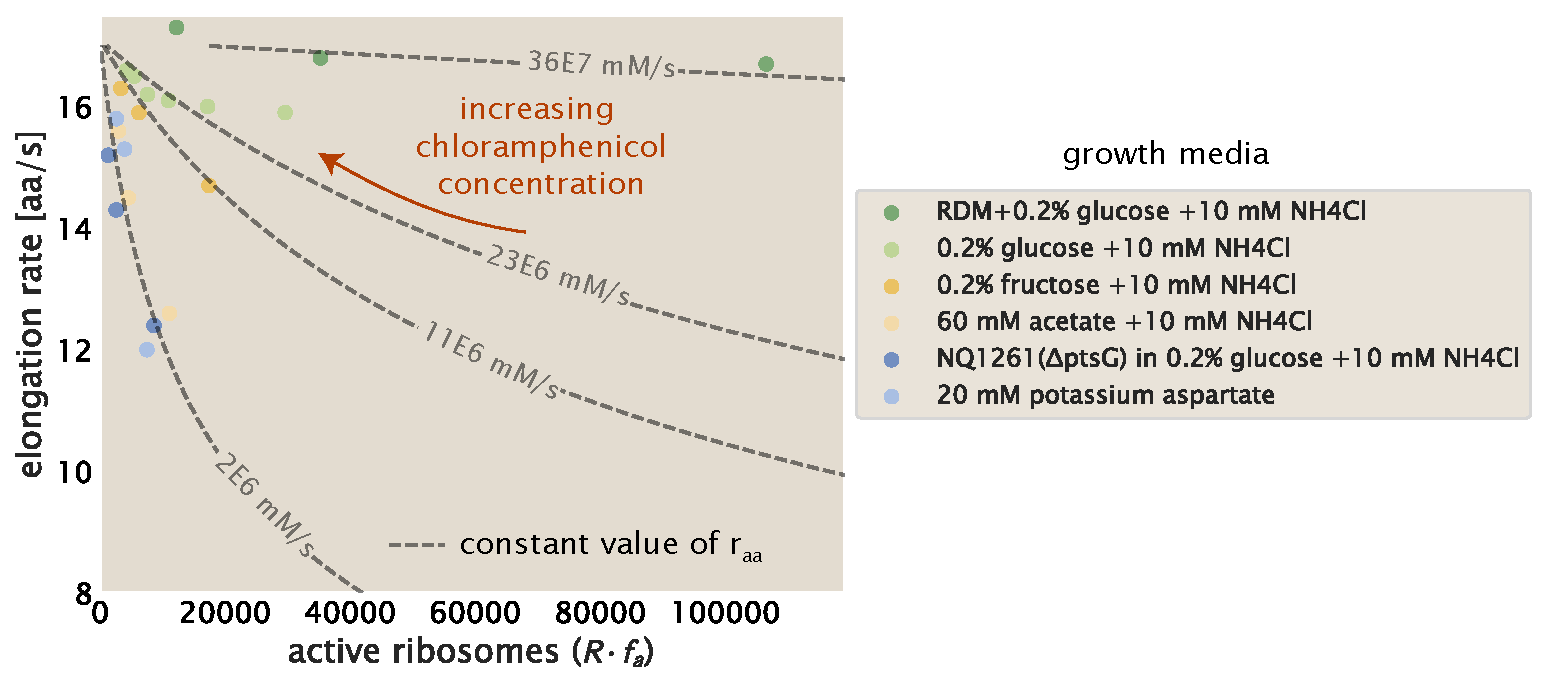
\includegraphics[width=0.8\textwidth]{SI_figs/SI_Dai_Cm.pdf}
        \caption{\textbf{.} }
        \label{fig:Dai_data_Cm}
    }
\end{figure*}

Figure \ref{fig:Dai_data_Cm} shows this data, along with dashed lines of
constant $r_aa$ based on Equation \ref{eq:rt_roots}. Consistent with our
hypothesis, we find that the fraction of active ribosomes and elongation rate
vary along line of roughly constant $r_aa$ for each growth condition. This is
even though cells were found to increase their RNA-to-protein ratio with
increasing concentrations of chloramphenicol. One point of caution here is that
since the ribosomal fraction ($\propto$ R_m/P_m ratio) was found to vary with
chloramphenicol concentration, other changes in the proteomic composition are
expected and it is unclear whether this might lead to a different value of
$r_aa$. Further experimental work would be needed to more carefully test our
predictions under perturbations like that performed with chloramphenicol.

As a final point, it is now possible to consider how the translation-limited
growth rate  might vary as the parameters $R, f_a$, and $r_t$ by using Equation
1 from the main text. This is re-written here for convienence,

\begin{equation}
\lambda_{\textrm{translation-limited}} \approx \frac{ln(2) \cdot r_t}{L_R}  \Phi_R.
\end{equation}
In the slow growth regime ($\appox$ 0.5 $hr^{-1}$ or slower), $\Phi_R$ does not
vary as dramatically as at fast growth and  in Figure 7(E) of the main text we
created a heatmap of growth rate across this parameter space by assuming a
constant value $\Phi_R$=0.13.
